\chapter{Methodology}
\section{Mechanism/Algorithm}
\begin{description}
   \item[1. Selections of the Sectors and Stocks] First, the present analysis will focus on nine crucial NSE sectors. Some industries include \emph{pharmaceuticals, infrastructure, real estate, media, public sector banks, private sector banks, and large-cap, mid-cap, and small-cap companies}. The leading stocks in each sector and their relative contributions to the calculation of the overall sectoral index are included in monthly reports published by the NSE.
The contributions are given percentage weights. D  determined using the NSE report released on Nov 31, 2023 \cite{NSEJune2022}. Following these actions, 28 stocks are picked for the nine specified industries.
   \item[2. Data Gathering] The download function provided by the Python language's yfinance module is used to retrieve the historical prices of its 28 equities from the Yahoo Finance website. The stock prices are utilised for portfolio creation for 23 years, beginning on January 1, 2000, and ending in Nov 2023. Six elements of the web-extracted raw data are open, high, low, close, volume, and adjusted close. The other factors are neglected since the present study is based on univariate analysis, which only considers the stock's closing price for the period from January 1, 2000, to Nov, 30 2023.
   \item[3. Volatility and Return on Investment] Each stock's return and log return values are calculated daily based on the relative historical values of that stock. The change in the closing values over consecutive days is expressed by the daily return and the log return for a stock, and their logarithms are calculated in percentage terms. Using Python's pct change library function, the daily return and log returns are calculated. The values of each stock's daily and annual volatility are then calculated. A stock's daily volatility is the standard deviation of its daily returns. The volatility numbers are computed using the Python function std. Given that there are 254 working days in a year, the daily volatility of a stock is multiplied by the square root of 254 to get its annual volatility. According to an investor's perspective, a stock's annual volatility is a sign of how risky it is.
   \item[4. Stock Return Covariance and Correlation Matrices] After obtaining each stock's return and volatility values, the stocks' covariance and correlation matrices are created based on their return values in the training dataset.  These matrices provide vital info for the creation of a portfolio by assisting in comprehending the patterns of relationship among the stocks in a specific sector. Python methods called cov and corr are used to calculate the covariance and correlation matrices. The main optimisation goals of a portfolio design work are minimising risk and optimisation. The algorithm tries to distribute funds across stocks with little or no correlation in a diversified portfolio that minimises risk. It is feasible to identify these stocks by examining their covariance or correlation matrices.
   \item[5. Portfolio Return and Risk Estimation] The first set of portfolios is built at this stage using each sector's covariance and correlation matrices. The portfolios are first created by giving each of the 28 stocks in a particular sector the same weight. The equal-weighted portfolio's annual return and volatility numbers are calculated for each of the nine sectors. The anticipated return of a portfolio made up of n capital assets (i.e., stocks) is indicated as Exp(Ret) in (Eq 1), from which the return of a portfolio based on its historical return values is calculated. 
   \[Exp(Ret) = w_{1}E(Ret_{c_{1}}) + w_{2}E(Ret_{c_{2}}) + ... w_{n}E(Ret_{c_{n}}) \qquad \textit{(Eq 1)}\] 
   The annual return and volatility of the equal-weight portfolio of each sector are calculated using the stock's annual return and volatility metrics. The mean annual returns for each stock that makes up a portfolio are calculated using the Python function which is resembled by argument 'Y'.
On the other hand, the daily volatility values are multiplied by a factor of the square root of 254 to obtain the annual volatility values for the equal-weight portfolios. The equal-weight portfolios serve as benchmarks for assessing the performance of other portfolios and provide one a baseline level of return and risk associated with the sectors over the training records. The return and risk projections made using equal-weighted portfolios, however, are very inaccurate predictors of future returns and dangers. Therefore, more accurate projections of the potential return and hazards are required.
The creation of the portfolios with the lowest and highest levels of risk is necessary as a result.
   \item[6. Designing Minimum-Risk Portfolios] At this stage, minimum-risk portfolios are created for the nine sectors to enhance the equal-weight portfolios.
The lowest values for their variances are seen in portfolios with the lowest risk. A particular portfolio's variance, $Variance(P)$, depends on the variances of the stocks that make up the portfolio as well as the covariances between each pair, as shown by (Eq 2).
\[Variance(P) = \sum_{i = 1}^{n} w_{i}s_{i}^2 + 2*\sum_{i,j}w_{i}*w_{j}*Covar(i,j)\qquad(Eq 2)\]
In (Eq 2), the weight given to stock $i$ is defined by $w_{i}$, the covariance between stocks is obtained by $Covar(i,j)$, and the volatility of the stock is determined by its standard deviation which is represented by $s_{i}$. Each portfolio has 28 stocks, hence 784 terms are needed to calculate each portfolio's variance. While the remaining 756 items represent the covariances between each pair, only 28 of the terms are included in the weighted sum of the variances of the individual stocks. The portfolio with the lowest risk is the one that can identify the set of ${w_{i}}'s$ that results in the portfolio's volatility being at its lowest value.\\\\

In order to determine which portfolio has the lowest risk for each sector, the \textit{efficient frontier (EF)} employing many portfolios is first presented. The returns and volatility are shown along the y-axis and the x-axis, respectively, in the two-dimensional plot of a set of portfolios in the EF. The EF frontier is composed of the portfolio in the form of points that provide the highest level of return of a given volatility or the lowest volatility for a given level of return. The point at the furthest left position on the EF represents the portfolio with the least volatility and, as a consequence, the lowest risk. The efficient frontier is drawn by 5000 iterations of a Python programme looping through a portfolio of equities, randomly allocating weights to each item. Every one of the 5,000 points that the algorithm produces corresponds to a portfolio with a certain return and risk value. The EF points are those that provide the lowest volatility for a given return value or the highest return value for a given volatility.

The portfolio with the lowest risk is represented by the leftmost location on the EF out of all the produced points.
\item [7.  Designing Optimum-Risk Portfolios] The investors in the stock market rarely follow the
strategy of risk minimisation as proposed by the minimum-
risk portfolio due to their low returns. Most often, the
investors are ready to undertake higher risks if the associated
returns are even higher. For optimising the risk and return in
a portfolio, and thereby designing an optimum-risk portfolio.
When compared to the minimum-risk portfolio, the optimum-risk portfolio generates a very high return with a hardly noticeable increase in risk.

\item [8. Back Testing the Strategy] A minimal risk portfolio and an optimum risk portfolio are developed for the sectors using the training information from January 1, 2000, to Nov 30, 2023. On Nov 30, 2023, a fictional investor is established who invests a sum of one million Indian rupees (INR) in each sector in accordance with the advice of the best risk-weighted portfolio structure for that sector. Please take note that the figure of INR 1 million is just meant to serve as an example. The quantity or the currency will have no impact on the analysis. A model is created utilising the Differen architectures to calculate the future stock price values and, in turn, estimate the future value of the portfolio. The expected rate of return for each portfolio is calculated using the predicted stock weights. Finally, the real rate of return is calculated on Nov 30, 2023, when the stock values are known. To assess the profitability of the portfolios and the model's predictive power, the anticipated and actual rates of return for each portfolio are compared.
\end{description}

\subsection{Model Architecture}

Figure~\ref{fig:network_architecture1} illustrates our model's structure. It consists of three primary components: an input layer, a processing layer utilizing a neural network, and an output layer. This architecture leverages neural networks to extract cross-sectional features from input data, aligning with research suggesting superior performance of deep learning features compared to traditional hand-crafted ones \citep{Zhang202025}. Following feature extraction, the model generates portfolio weights used to calculate returns and maximize the Sharpe ratio. 
\begin{figure}[H]
   \centering
   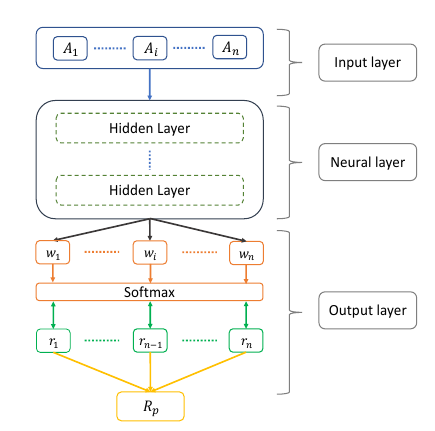
\includegraphics[width=0.5\linewidth]{images/model_schema.png}
   \caption{Model architecture schematic}
   \label{fig:network_architecture1}
 \end{figure}
 
\subsection{Detailed Breakdown}

\subsubsection{Input Layer}

Each asset (represented as $A_i$) is part of a portfolio containing $n$ assets. We combine data from all assets into a single input. This input could be historical prices and returns for one asset, with a dimension of $(k, 2)$ where $k$ represents the lookback window. Stacking features across all assets would result in a dimension of $(k, 2 \times n)$. This input is then fed into the network for extracting non-linear characteristics.

\subsubsection{Processing Layer (Neural Network)}

This layer can be built by stacking multiple hidden layers. However, designing this layer requires experimentation as various hidden layer combinations exist, and performance often hinges on the architecture's design. We explored Long Short-Term Memory (LSTM), Convolutional Neural Networks (CNN), and Fully Connected Neural Networks (FCN) \citep{Hochreiter19971735}. Studies suggest LSTMs achieve the best overall performance for daily financial data modeling (\citep{8081663}, \citep{lim2020enhancing}).

\begin{itemize}
    \item \textbf{Fully Connected Neural Networks (FCNs):} A major concern with FCNs is their tendency to overfit due to the large number of parameters assigned to each input feature.
    \item \textbf{Long Short-Term Memory (LSTMs):} LSTMs utilize a cell structure with gate mechanisms to summarize and filter data from extended histories. This leads to fewer trainable parameters and improved generalization capabilities.
    \item \textbf{Convolutional Neural Networks (CNNs):} While CNNs excel at modeling high-frequency financial data (like limit order books), their smoothing properties (often associated with large convolutional filters) can generate overly smooth solutions. Additionally, the convolution process and parameter sharing architecture of CNNs can lead to overfiltering of inputs.
\end{itemize}

\subsubsection{Output Layer}

To create a long-only portfolio, we employ the softmax activation function in the output layer. This function inherently enforces constraints, ensuring portfolio weights are positive and sum to one. Since the number of output nodes $(w_1, w_2, ..., w_n)$ corresponds to the number of assets $(n)$ in the portfolio, these weights can be multiplied by the respective asset returns $(r_1, r_2, ..., r_n)$ to obtain the realized portfolio return ($R_p$). With the realized returns, we can calculate the gradients of the Sharpe ratio concerning the model's parameters and utilize gradient ascent for parameter updates.

\label{fig:network_architecture}


\chapter{Experiments and Results}

This chapter delves into the experiments conducted to evaluate the proposed hypothesis regarding a system that achieves a favorable reward-to-risk ratio. As a diversified portfolio is known to yield a better return per unit of risk, our approach aims to achieve this objective.

\section{Dataset Description}

The dataset employed in this study encompasses daily measurements from 2000 to 2024. We leverage this data to train and update our model parameters on a quarterly basis. The testing period spans from 2000 to Mar 2024, encompassing the recent economic crises associated with COVID-19. Citing a relevant source (e.g., [Source on economic impact of COVID-19]), you can elaborate on the specific challenges this period presented.

\begin{longtblr}[
  caption = {Summary statistics for close prices of assets used. },
]{
  width = \linewidth,
  colspec = {Q[333]Q[142]Q[142]Q[142]Q[162]},
  column{even} = {r},
  column{3} = {r},
  column{5} = {r},
  hlines,
  vlines,
  hline{1,52} = {-}{0.08em},
}
\textbf{Ticker} & \textbf{Mean} & \textbf{Std} & \textbf{Min} & \textbf{Max}\\
ADANIENT.NS & 1184.55 & 1172.52 & 66.39 & 4163.22\\
ADANIPORTS.NS & 571.20 & 238.63 & 203.57 & 1342.60\\
APOLLOHOSP.NS & 2923.24 & 1677.39 & 909.28 & 6774.05\\
ASIANPAINT.NS & 2267.77 & 814.44 & 1055.82 & 3537.52\\
AXISBANK.NS & 716.45 & 172.94 & 302.38 & 1136.95\\
BAJAJ-AUTO.NS & 3329.54 & 1201.65 & 1749.60 & 8879.05\\
BAJAJFINSV.NS & 1071.82 & 446.92 & 409.26 & 1905.96\\
BAJFINANCE.NS & 4800.36 & 2030.86 & 1572.28 & 8168.55\\
BHARTIARTL.NS & 573.86 & 223.25 & 251.85 & 1228.35\\
BPCL.NS & 327.44 & 65.46 & 184.11 & 657.60\\
BRITANNIA.NS & 3382.18 & 792.01 & 1960.17 & 5361.30\\
CIPLA.NS & 793.50 & 259.73 & 367.86 & 1504.10\\
COALINDIA.NS & 162.08 & 71.11 & 75.51 & 474.53\\
DIVISLAB.NS & 2810.15 & 1217.51 & 946.77 & 5288.63\\
DRREDDY.NS & 3876.79 & 1201.93 & 1815.33 & 6449.60\\
EICHERMOT.NS & 2610.77 & 632.66 & 1238.16 & 4180.35\\
GRASIM.NS & 1240.78 & 464.41 & 391.72 & 2254.90\\
HCLTECH.NS & 778.02 & 329.68 & 353.73 & 1686.40\\
HDFCBANK.NS & 1283.53 & 252.87 & 747.04 & 1728.20\\
HDFCLIFE.NS & 551.78 & 100.60 & 338.78 & 754.39\\
HEROMOTOCO.NS & 2676.20 & 505.14 & 1418.74 & 4882.53\\
HINDALCO.NS & 318.27 & 134.21 & 85.50 & 621.50\\
HINDUNILVR.NS & 2063.53 & 422.52 & 1145.88 & 2737.03\\
ICICIBANK.NS & 592.91 & 244.27 & 253.10 & 1097.10\\
INDUSINDBK.NS & 1206.32 & 379.16 & 294.20 & 1964.97\\
INFY.NS & 1073.85 & 431.62 & 415.89 & 1849.31\\
ITC.NS & 254.74 & 90.09 & 122.58 & 485.03\\
JSWSTEEL.NS & 471.01 & 223.96 & 133.18 & 880.80\\
KOTAKBANK.NS & 1594.93 & 288.50 & 994.99 & 2207.80\\
LT.NS & 1623.30 & 652.71 & 670.62 & 3708.00\\
LTIM.NS & 3348.09 & 1760.15 & 891.71 & 7385.38\\
M & M.NS & 886.17 & 357.55 & 259.47\\
MARUTI.NS & 7732.31 & 1405.22 & 3888.12 & 11670.60\\
NESTLEIND.NS & 1575.34 & 490.43 & 642.01 & 2729.54\\
NTPC.NS & 128.48 & 56.84 & 62.65 & 358.25\\
ONGC.NS & 118.89 & 40.56 & 44.61 & 283.75\\
POWERGRID.NS & 116.89 & 47.50 & 63.90 & 295.00\\
RELIANCE.NS & 1749.04 & 604.25 & 785.60 & 3014.80\\
SBILIFE.NS & 959.66 & 262.82 & 505.41 & 1549.77\\
SBIN.NS & 384.53 & 145.95 & 144.37 & 788.05\\
SUNPHARMA.NS & 692.27 & 280.80 & 311.44 & 1605.70\\
TATACONSUM.NS & 547.51 & 270.32 & 172.19 & 1261.55\\
TATAMOTORS.NS & 340.66 & 190.58 & 65.10 & 1039.30\\
TATASTEEL.NS & 75.80 & 36.64 & 22.23 & 157.25\\
TCS.NS & 2583.87 & 797.49 & 1120.03 & 4207.60\\
TECHM.NS & 874.99 & 303.96 & 390.43 & 1686.90\\
TITAN.NS & 1762.82 & 859.67 & 736.47 & 3866.65\\
ULTRACEMCO.NS & 5690.27 & 1856.12 & 2963.37 & 10503.05\\
UPL.NS & 575.40 & 128.48 & 241.14 & 818.25\\
WIPRO.NS & 360.44 & 135.82 & 159.65 & 711.11
\end{longtblr}

\section{Evaluation Metrics}

\subsection{Expected Return}
Expected return is a fundamental metric in portfolio optimization, representing the mean value of potential profits or losses. It quantifies the average gain or loss an investor anticipates from an investment over a specific period. Higher expected returns generally indicate greater potential for profitability, albeit often with increased risk.

\subsection{Volatility}
Volatility measures the degree of variation in investment returns over time. It reflects the dispersion of possible outcomes and is a key indicator of investment risk. High volatility suggests greater price fluctuations and higher risk, while low volatility indicates more stable returns but potentially lower profits.

\subsection{Max Drawdown}
Max drawdown refers to the maximum decline in portfolio value from its peak to its lowest point. It is a crucial metric for assessing risk tolerance and potential losses during adverse market conditions. Minimizing max drawdown helps investors preserve capital and maintain long-term portfolio growth.

\subsection{Sharpe Ratio}
The Sharpe ratio evaluates the risk-adjusted return of an investment by comparing the excess return to the standard deviation of returns. A higher Sharpe ratio indicates better risk-adjusted performance, with greater returns relative to the level of risk undertaken.

\subsection{Sortino Ratio}
The Sortino ratio is a variation of the Sharpe ratio that focuses on downside risk. It measures the excess return per unit of downside deviation, providing a more targeted assessment of risk-adjusted returns. A higher Sortino ratio signifies superior performance in generating returns while minimizing downside volatility.

\subsection{Omega Ratio}
The Omega ratio evaluates the probability-weighted average return relative to a specified target threshold. It considers both the magnitude and frequency of returns above or below the threshold, providing insight into the asymmetry of return distributions. A higher Omega ratio indicates a higher probability of achieving returns above the target threshold.

\subsection{CAGR}
The Compound Annual Growth Rate (CAGR) quantifies the geometric progression rate of an investment over a specified period, accounting for compounding effects. It provides a smoothed representation of growth, enabling meaningful comparisons of investment performance across different time frames. CAGR facilitates long-term investment planning by indicating the average annual growth rate required to reach a specified investment goal.

\section{Results}
\subsection{Equal-Weighted Portfolio Optimization}

\begin{figure}[H]
   \centering
   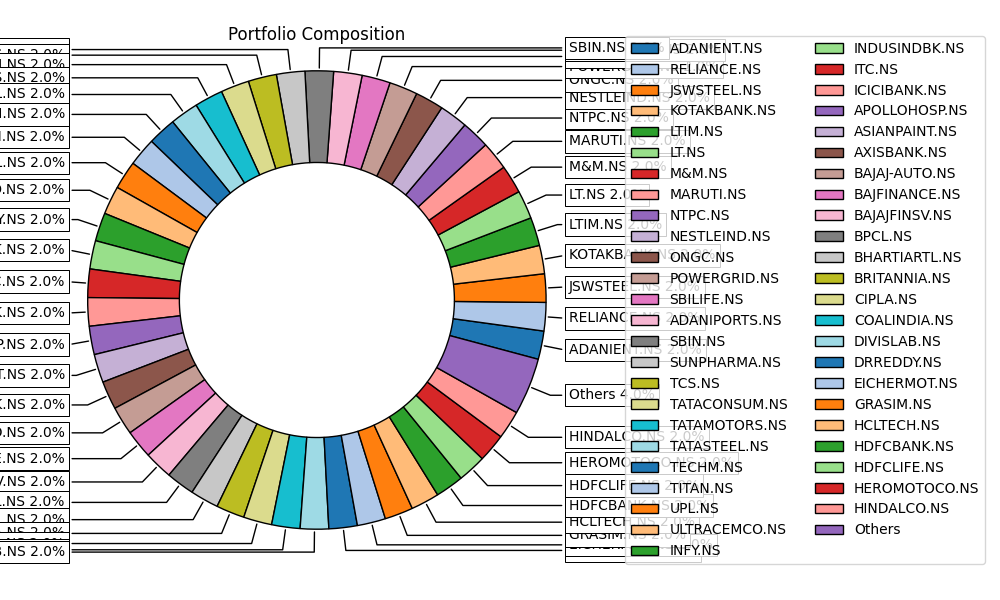
\includegraphics[width=1\linewidth]{images/equal_weight/Weights.png}
   \caption{Latest Weights from Optimization}
   \label{fig:network_architecture1}
 \end{figure}

 \begin{figure}[H]
   \centering
   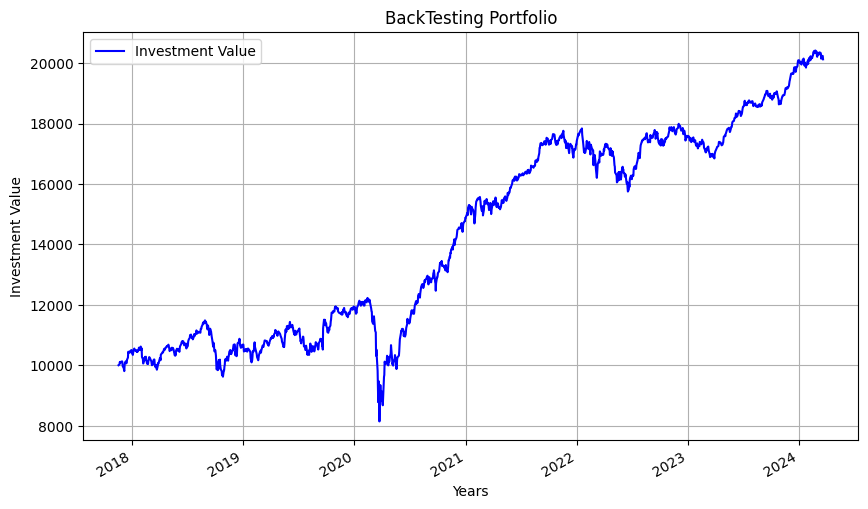
\includegraphics[width=1\linewidth]{images/equal_weight/backtest.png}
   \caption{Backtesting Result}
   \label{fig:network_architecture1}
 \end{figure}

 \begin{table}[H]

    \centering % instead of \begin{center}
    \label{tab:performance_metrics}
    
    \caption{Performace Metrics}
    \vspace{5mm} % Adjust the height of the space between caption and tabular

\begin{tabular}{lr}
\toprule
 & Results \\
\midrule
Expected Return & 16.31\% \\
Volatility & 17.63\% \\
Max Drawdown & -35.01\% \\
Sharpe Ratio & 0.93 \\
Sortino Ratio & 276.23 \\
Omega Ratio & 14.92 \\
CAGR & 15.89\% \\
\bottomrule
\end{tabular}
\end{table}

\subsection{Maximum Diversification Portfolio Optimization}

\begin{figure}[H]
   \centering
   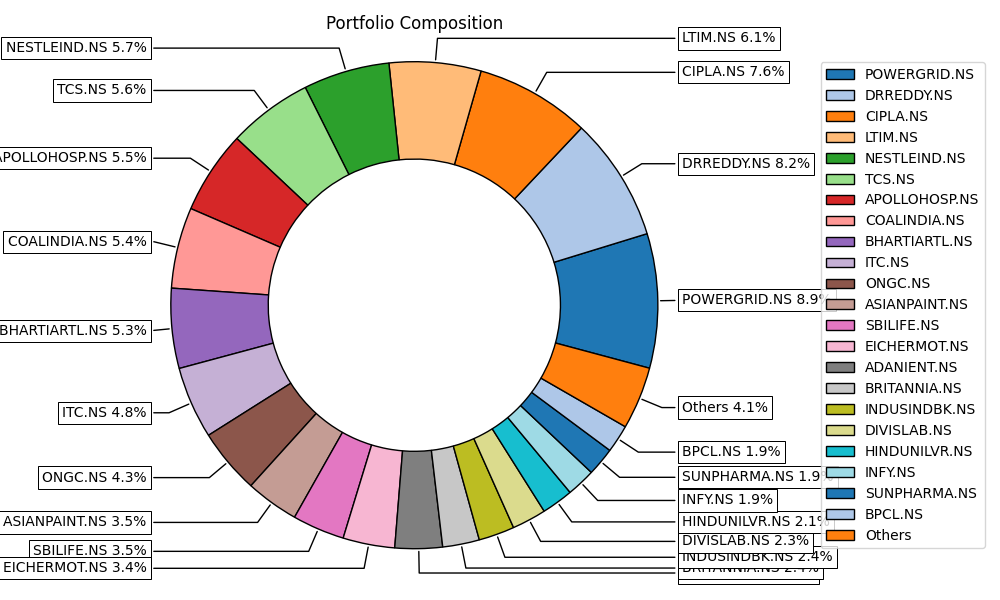
\includegraphics[width=1\linewidth]{images/Max_diver/Weights.png}
   \caption{Latest Weights from Optimization}
   \label{fig:network_architecture1}
 \end{figure}

 \begin{figure}[H]
   \centering
   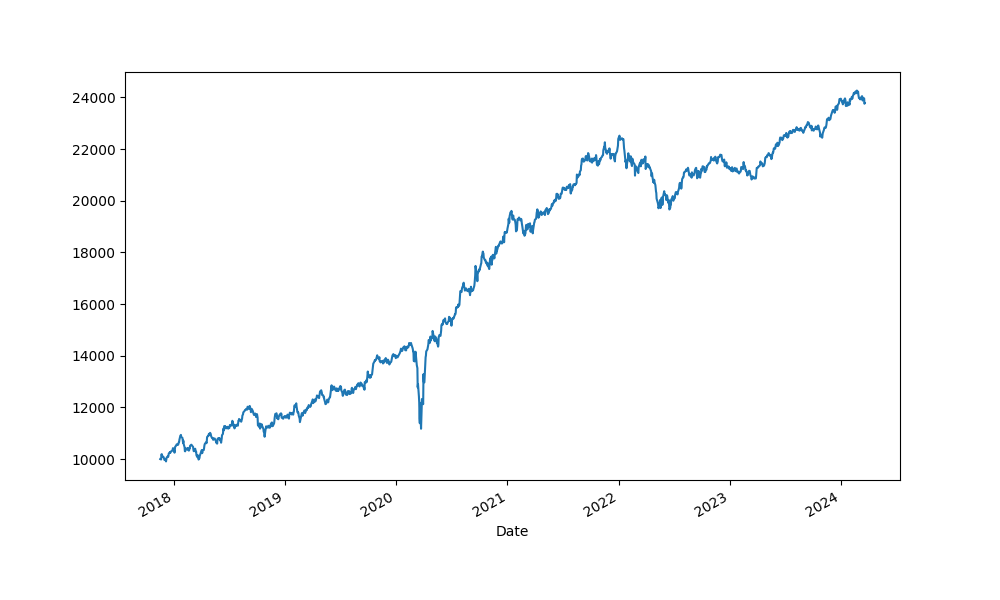
\includegraphics[width=1\linewidth]{images/Max_diver/backtest.png}
   \caption{Backtesting Result}
   \label{fig:network_architecture1}
 \end{figure}

 \begin{table}[H]

    \centering % instead of \begin{center}
    \label{tab:performance_metrics}
    
    \caption{Performace Metrics}
    \vspace{5mm} % Adjust the height of the space between caption and tabular

\begin{tabular}{lr}
\toprule
 & Results \\
\midrule
Expected Return & 22.20\% \\
Volatility & 17.40\% \\
Max Drawdown & -29.48\% \\
Sharpe Ratio & 1.28 \\
Sortino Ratio & 424.15 \\
Omega Ratio & 16.18 \\
CAGR & 22.98\% \\
\bottomrule
\end{tabular}
\end{table}

\subsection{Risk Parity Portfolio Optimisation}

\begin{figure}[H]
   \centering
   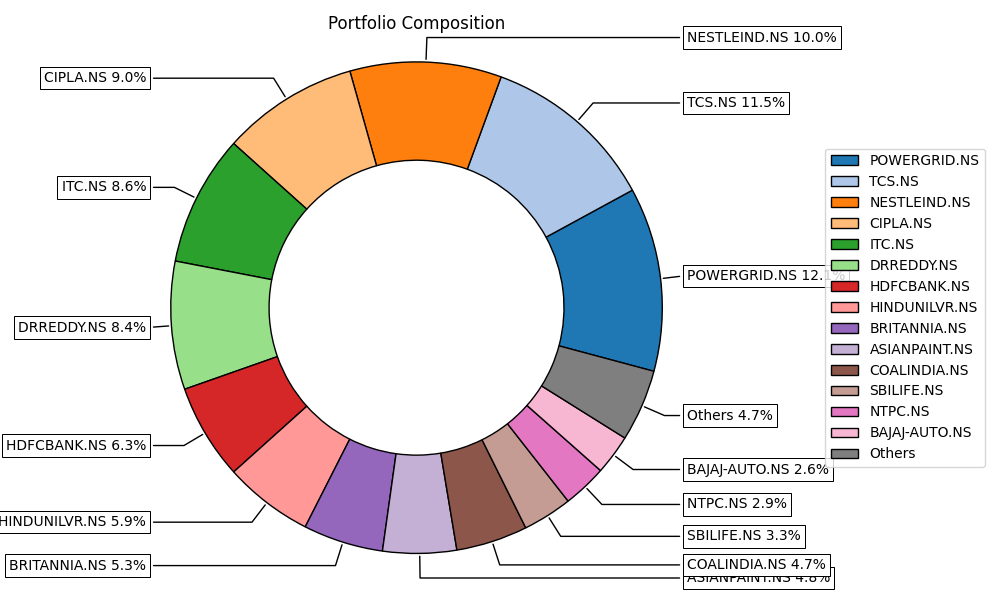
\includegraphics[width=1\linewidth]{images/risk_parity/Weights.png}
   \caption{Latest Weights from Optimization}
   \label{fig:network_architecture1}
 \end{figure}

 \begin{figure}[H]
   \centering
   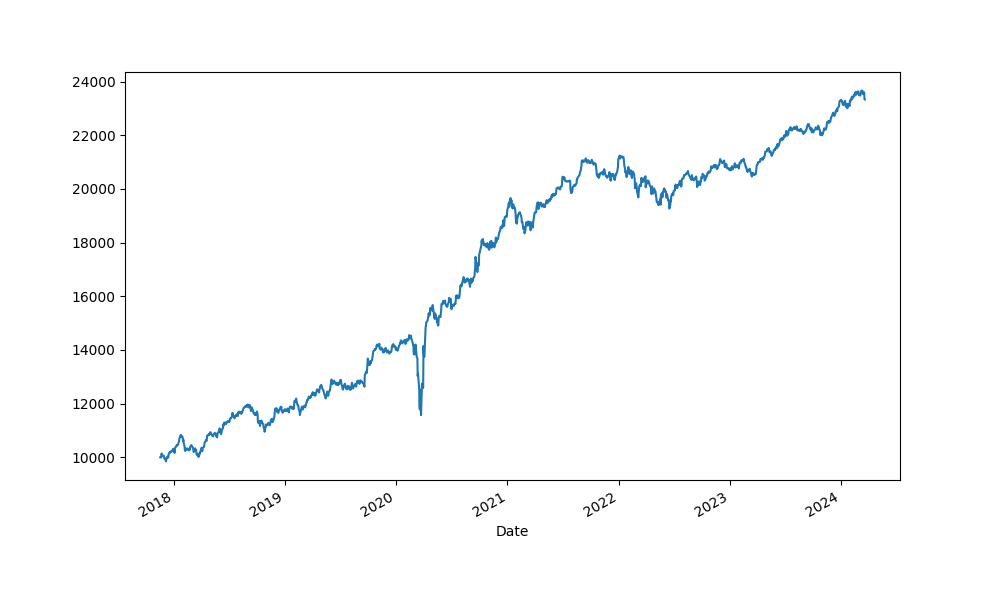
\includegraphics[width=1\linewidth]{images/risk_parity/backtest.png}
   \caption{Backtesting Result}
   \label{fig:network_architecture1}
 \end{figure}

 \begin{table}[H]

    \centering % instead of \begin{center}
    \label{tab:performance_metrics}
    
    \caption{Performace Metrics}
    \vspace{5mm} % Adjust the height of the space between caption and tabular

\begin{tabular}{lr}
\toprule
 & Results \\
\midrule
Expected Return & 21.47\% \\
Volatility & 16.91\% \\
Max Drawdown & -26.83\% \\
Sharpe Ratio & 1.27 \\
Sortino Ratio & 443.91 \\
Omega Ratio & 15.95 \\
CAGR & 22.20\% \\
\bottomrule
\end{tabular}
\end{table}

\subsection{Mean-Absolute Deviation Portfolio Optimisation}

\begin{figure}[H]
   \centering
   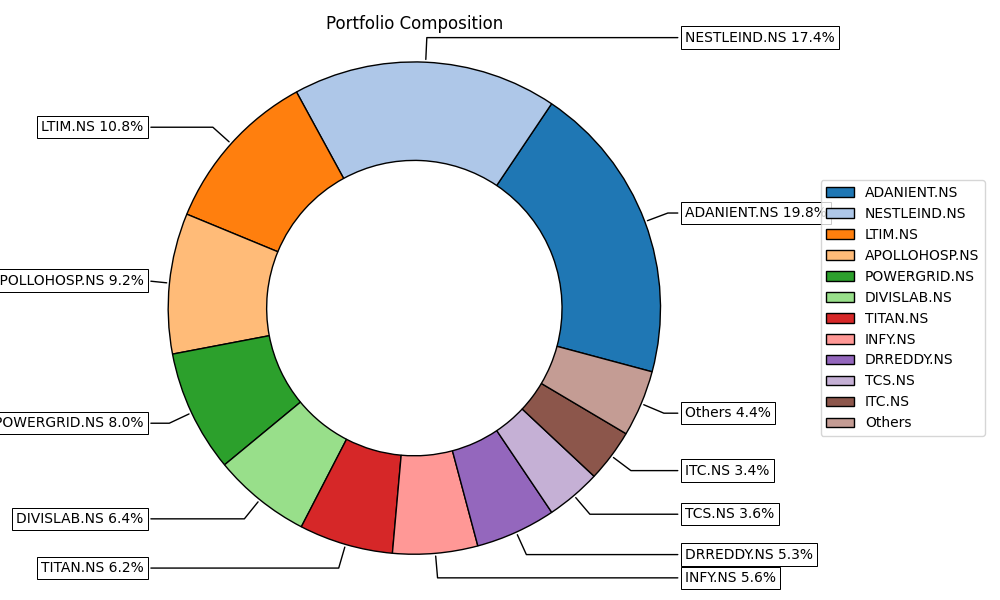
\includegraphics[width=1\linewidth]{images/MAD/Weights.png}
   \caption{Latest Weights from Optimization}
   \label{fig:network_architecture1}
 \end{figure}

 \begin{figure}[H]
   \centering
   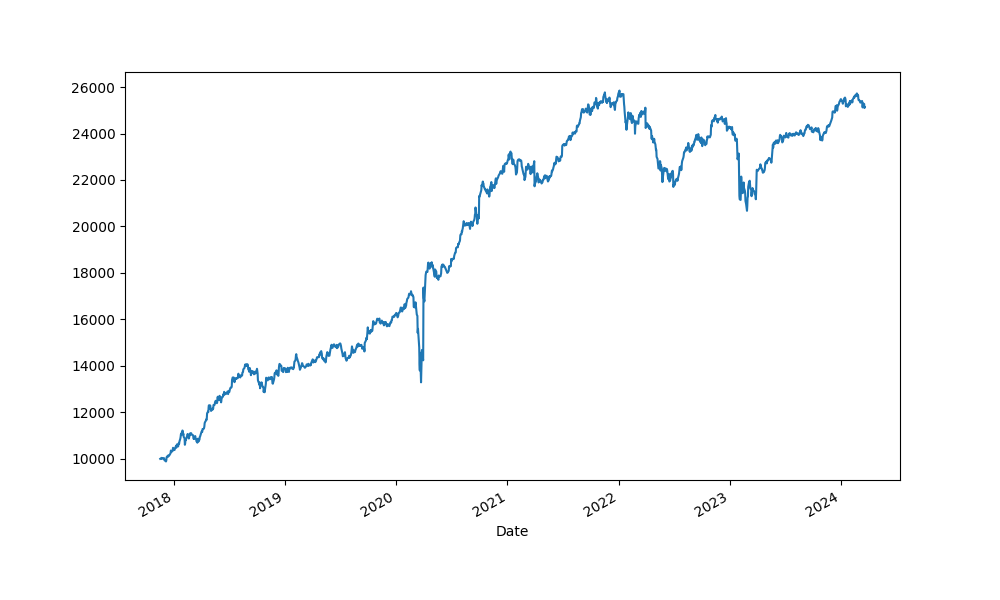
\includegraphics[width=1\linewidth]{images/MAD/backtest.png}
   \caption{Backtesting Result}
   \label{fig:network_architecture1}
 \end{figure}

 \begin{table}[H]

    \centering % instead of \begin{center}
    \label{tab:performance_metrics}
    
    \caption{Performace Metrics}
    \vspace{5mm} % Adjust the height of the space between caption and tabular

\begin{tabular}{lr}
\toprule
 & Results \\
\midrule
Expected Return & 24.37\% \\
Volatility & 25.80\% \\
Max Drawdown & -43.27\% \\
Sharpe Ratio & 0.94 \\
Sortino Ratio & 313.08 \\
Omega Ratio & 15.23 \\
CAGR & 23.55\% \\
\bottomrule
\end{tabular}
\end{table}

\subsection{Minimax Portfolio Optimisation}

\begin{figure}[H]
   \centering
   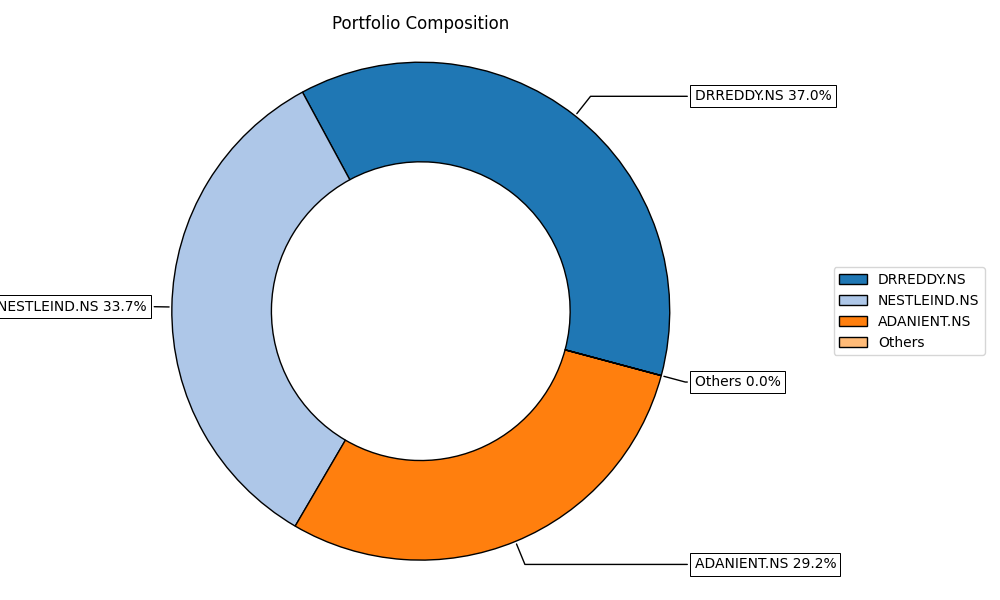
\includegraphics[width=1\linewidth]{images/minimax/Weights.png}
   \caption{Latest Weights from Optimization}
   \label{fig:network_architecture1}
 \end{figure}

 \begin{figure}[H]
   \centering
   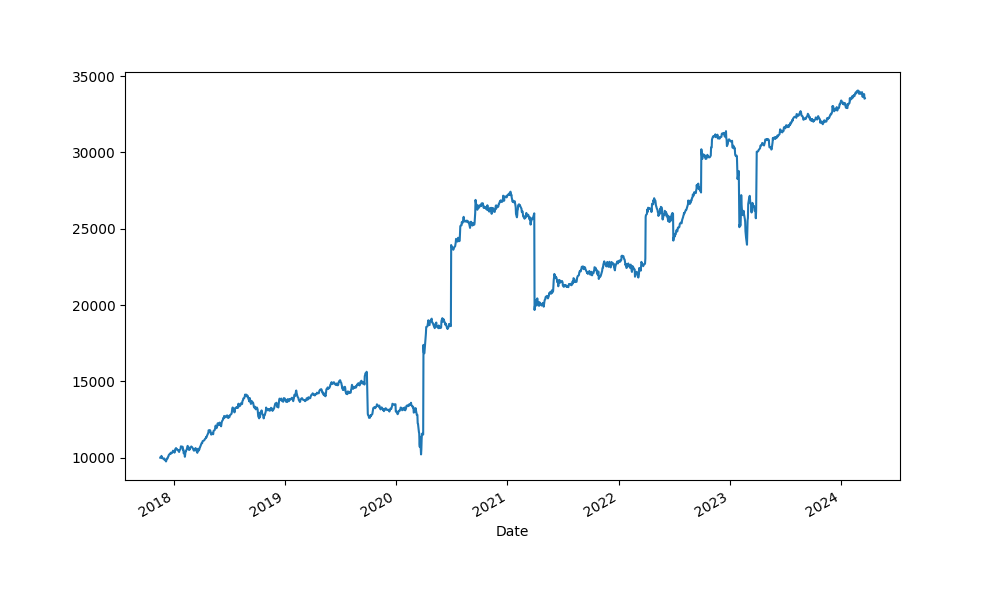
\includegraphics[width=1\linewidth]{images/minimax/backtest.png}
   \caption{Backtesting Result}
   \label{fig:network_architecture1}
 \end{figure}

 \begin{table}[H]

    \centering % instead of \begin{center}
    \label{tab:performance_metrics}
    
    \caption{Performace Metrics}
    \vspace{5mm} % Adjust the height of the space between caption and tabular

\begin{tabular}{lr}
\toprule
 & Results \\
\midrule
Expected Return & 37.90\% \\
Volatility & 55.27\% \\
Max Drawdown & -68.39\% \\
Sharpe Ratio & 0.69 \\
Sortino Ratio & 198.81 \\
Omega Ratio & 16.68 \\
CAGR & 23.88\% \\
\bottomrule
\end{tabular}
\end{table}

\subsection{Mean Variance Portfolio Optimisation}

\begin{figure}[H]
   \centering
   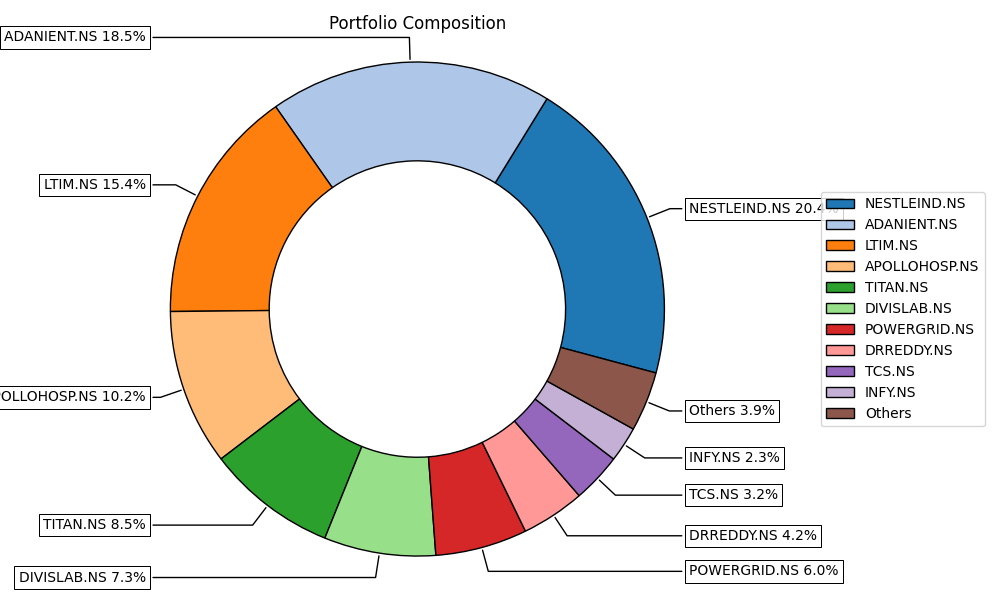
\includegraphics[width=1\linewidth]{images/MV/Weights.png}
   \caption{Latest Weights from Optimization}
   \label{fig:network_architecture1}
 \end{figure}

 \begin{figure}[H]
   \centering
   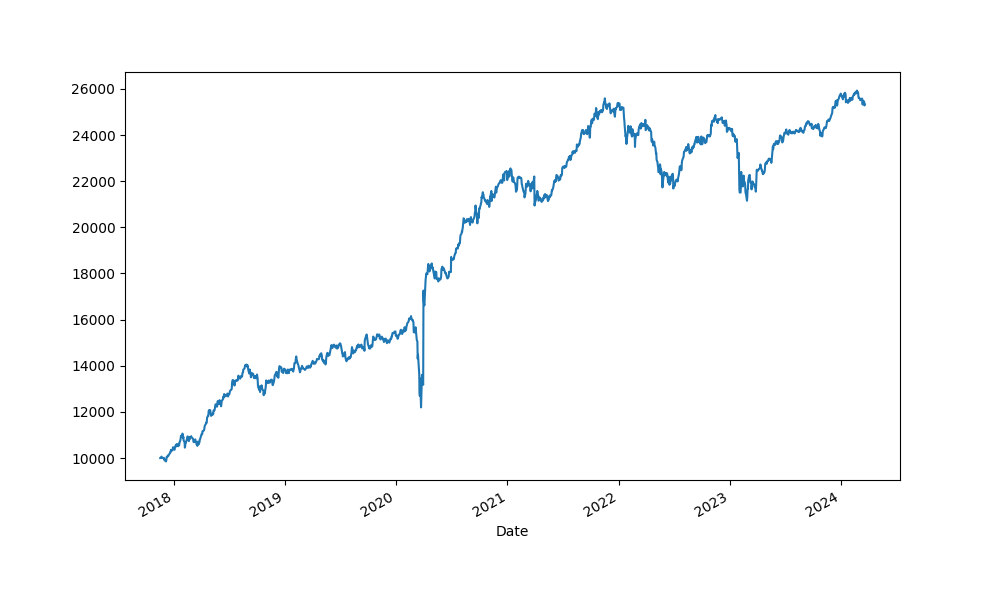
\includegraphics[width=1\linewidth]{images/MV/backtest.png}
   \caption{Backtesting Result}
   \label{fig:network_architecture1}
 \end{figure}

 \begin{table}[H]

    \centering % instead of \begin{center}
    \label{tab:performance_metrics}
    
    \caption{Performace Metrics}
    \vspace{5mm} % Adjust the height of the space between caption and tabular

\begin{tabular}{lr}
\toprule
 & Results \\
\midrule
Expected Return & 24.68\% \\
Volatility & 27.69\% \\
Max Drawdown & -38.75\% \\
Sharpe Ratio & 0.89 \\
Sortino Ratio & 323.36 \\
Omega Ratio & 15.47 \\
CAGR & 23.48\% \\
\bottomrule
\end{tabular}
\end{table}

\subsection{Lower Partial Moment Portfolio Optimisation}

\begin{figure}[H]
   \centering
   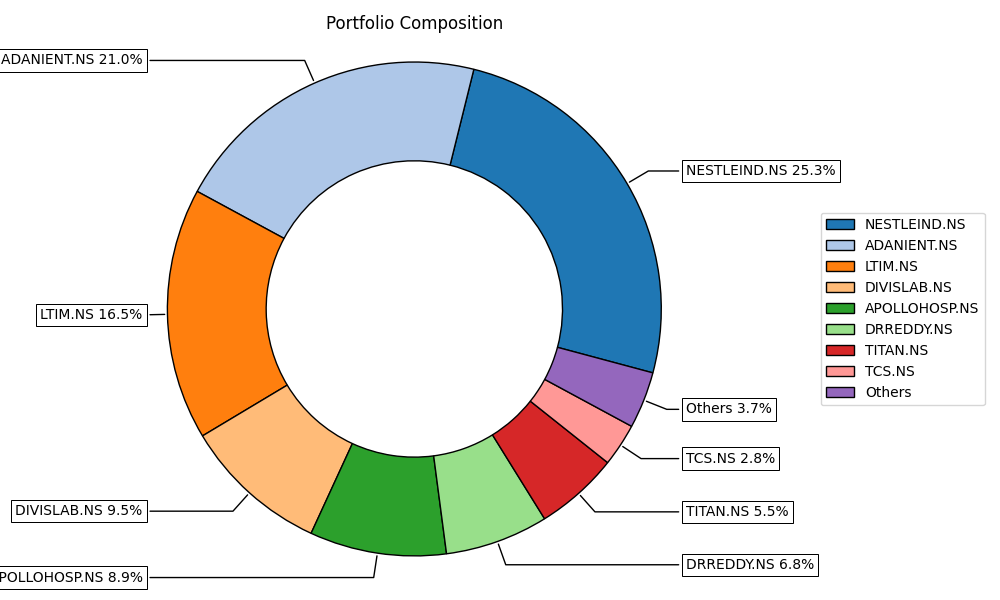
\includegraphics[width=1\linewidth]{images/LPM/Weights.png}
   \caption{Latest Weights from Optimization}
   \label{fig:network_architecture1}
 \end{figure}

 \begin{figure}[H]
   \centering
   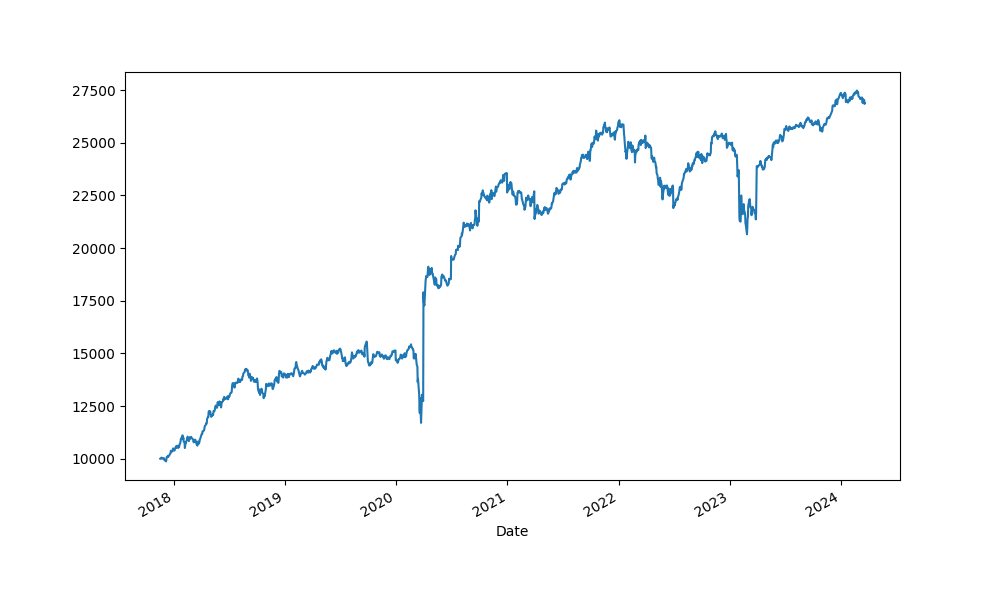
\includegraphics[width=1\linewidth]{images/LPM/backtest.png}
   \caption{Backtesting Result}
   \label{fig:network_architecture1}
 \end{figure}

 \begin{table}[H]

    \centering % instead of \begin{center}
    \label{tab:performance_metrics}
    
    \caption{Performace Metrics}
    \vspace{5mm} % Adjust the height of the space between caption and tabular

\begin{tabular}{lr}
\toprule
 & Results \\
\midrule
Expected Return & 27.19\% \\
Volatility & 33.53\% \\
Max Drawdown & -45.41\% \\
Sharpe Ratio & 0.81 \\
Sortino Ratio & 305.74 \\
Omega Ratio & 15.78 \\
CAGR & 24.74\% \\
\bottomrule
\end{tabular}
\end{table}

\subsection{Random Forest (RF) Optimization}

\begin{figure}[H]
   \centering
   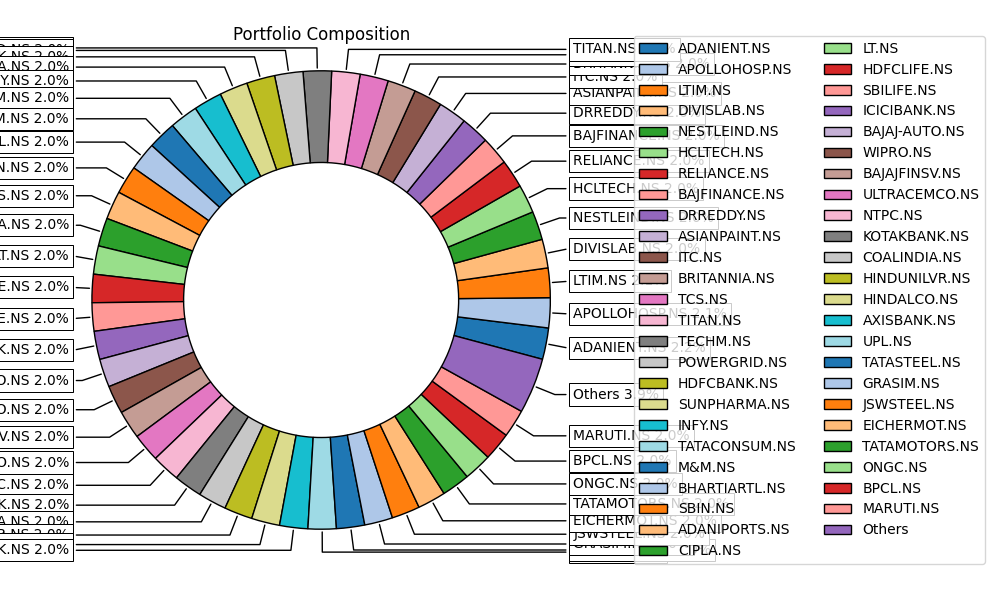
\includegraphics[width=1\linewidth]{images/RF/Weights.png}
   \caption{Latest Weights from Optimization}
   \label{fig:network_architecture1}
 \end{figure}

 \begin{figure}[H]
   \centering
   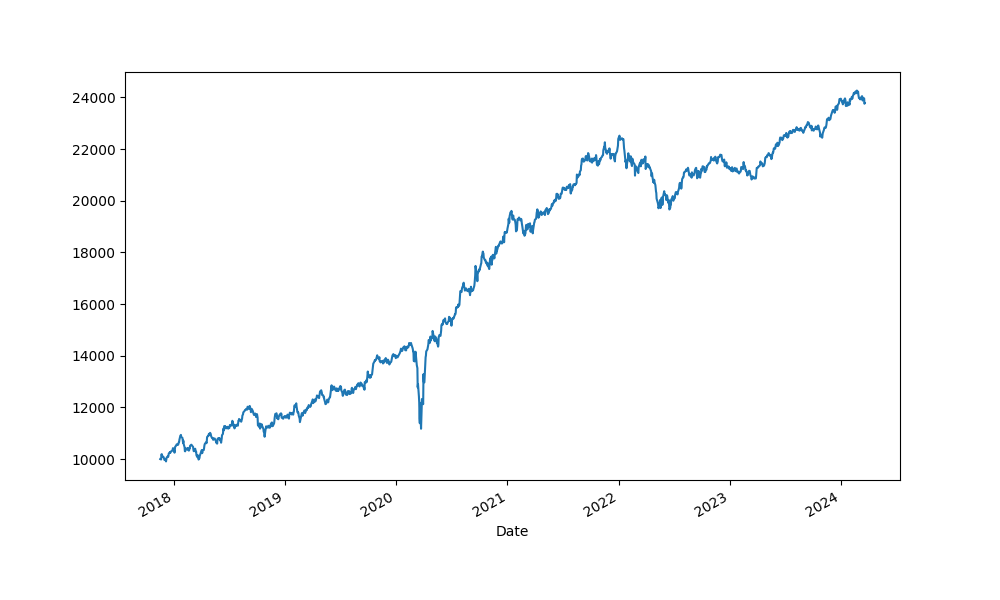
\includegraphics[width=1\linewidth]{images/Max_diver/backtest.png}
   \caption{Backtesting Result}
   \label{fig:network_architecture1}
 \end{figure}

 \begin{table}[H]

    \centering % instead of \begin{center}
    \label{tab:performance_metrics}
    
    \caption{Performace Metrics}
    \vspace{5mm} % Adjust the height of the space between caption and tabular

\begin{tabular}{lr}
\toprule
 & Results \\
\midrule
Expected Return & 22.20\% \\
Volatility & 17.40\% \\
Max Drawdown & -29.48\% \\
Sharpe Ratio & 1.28 \\
Sortino Ratio & 424.15 \\
Omega Ratio & 16.18 \\
CAGR & 22.98\% \\
\bottomrule
\end{tabular}
\end{table}

\subsection{Support Vector Regression (SVR) Optimization}

\begin{figure}[H]
   \centering
   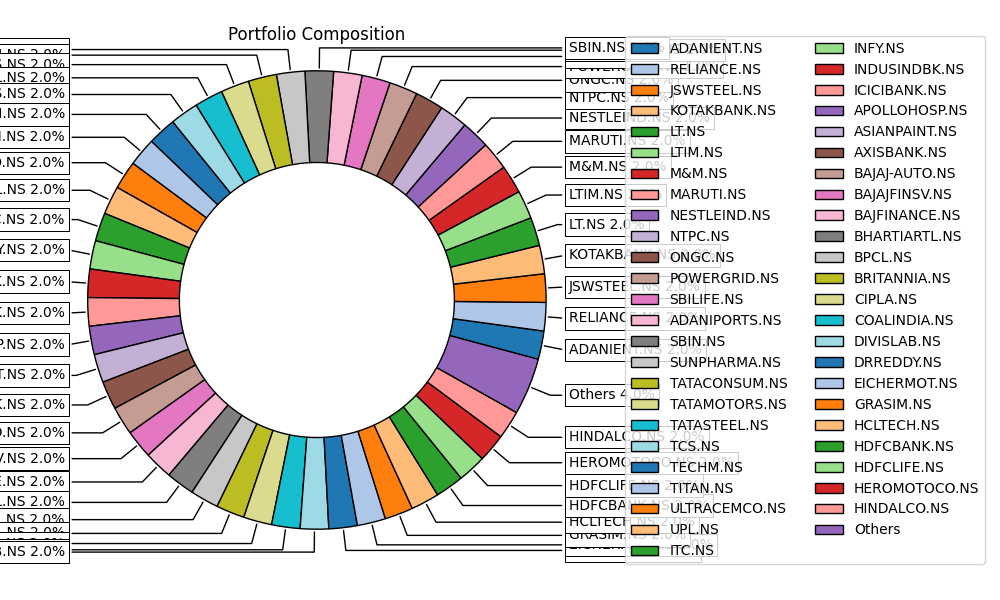
\includegraphics[width=1\linewidth]{images/SVM/Weights.png}
   \caption{Latest Weights from Optimization}
   \label{fig:network_architecture1}
 \end{figure}

 \begin{figure}[H]
   \centering
   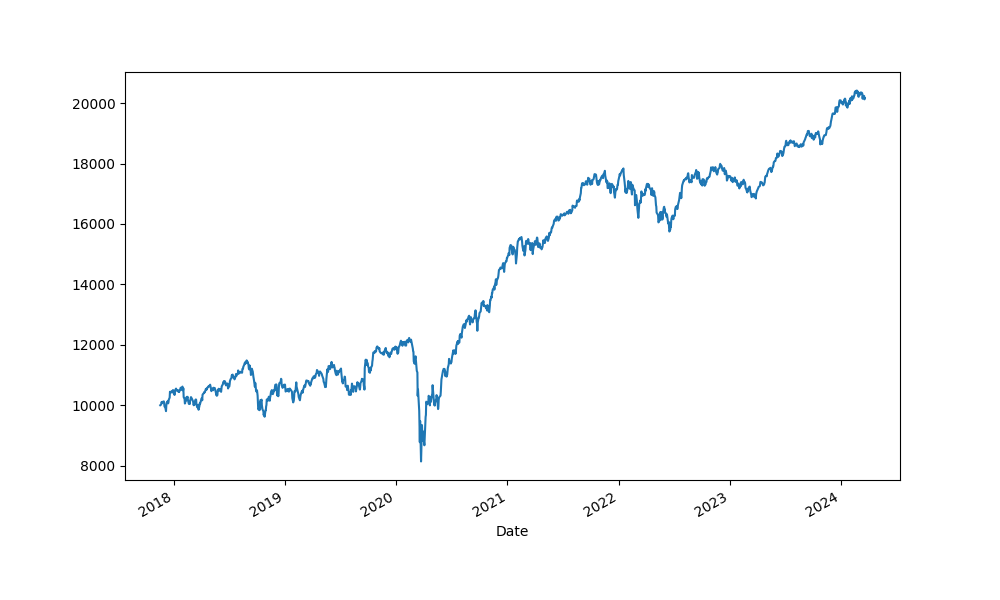
\includegraphics[width=1\linewidth]{images/SVM/backtest.png}
   \caption{Backtesting Result}
   \label{fig:network_architecture1}
 \end{figure}

 \begin{table}[H]

    \centering % instead of \begin{center}
    \label{tab:performance_metrics}
    
    \caption{Performace Metrics}
    \vspace{5mm} % Adjust the height of the space between caption and tabular

\begin{tabular}{lr}
\toprule
 & Results \\
\midrule
Expected Return & 16.38\% \\
Volatility & 17.62\% \\
Max Drawdown & -35.01 \\
Sharpe Ratio & 0.93 \\
Sortino Ratio & 277.27 \\
Omega Ratio & 14.91\% \\
CAGR & 15.96\% \\
\bottomrule
\end{tabular}
\end{table}

\subsection{Deep Multilayer Perceptron Optimization}

\begin{figure}[H]
   \centering
   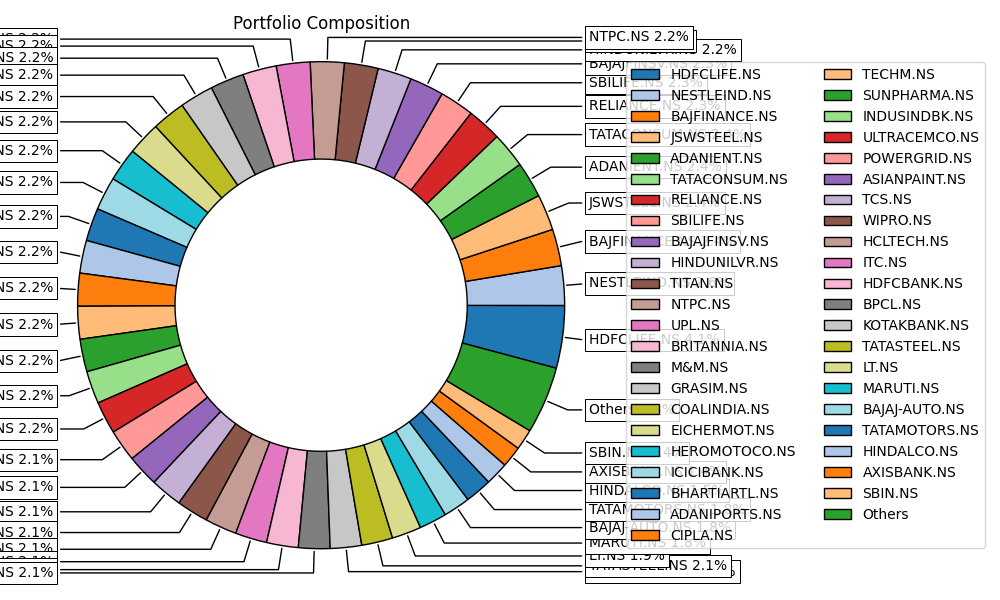
\includegraphics[width=1\linewidth]{images/DMLP/Weights.png}
   \caption{Latest Weights from Optimization}
   \label{fig:network_architecture1}
 \end{figure}

 \begin{figure}[H]
   \centering
   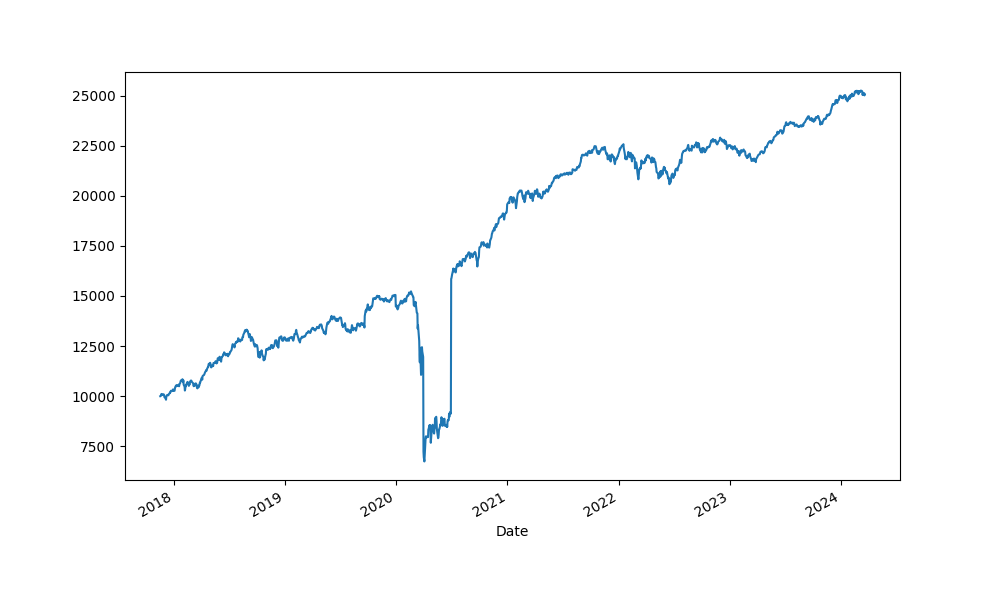
\includegraphics[width=1\linewidth]{images/DMLP/backtest.png}
   \caption{Backtesting Result}
   \label{fig:network_architecture1}
 \end{figure}

 \begin{table}[H]

    \centering % instead of \begin{center}
    \label{tab:performance_metrics}
    
    \caption{Performace Metrics}
    \vspace{5mm} % Adjust the height of the space between caption and tabular

\begin{tabular}{lr}
\toprule
 & Results \\
\midrule
Expected Return & 24.24\% \\
Volatility & 37.89\% \\
Max Drawdown & -64.77\% \\
Sharpe Ratio & 0.64 \\
Sortino Ratio & 187.36 \\
Omega Ratio & 15.18 \\
CAGR & 18.82\% \\
\bottomrule
\end{tabular}
\end{table}

\subsection{Long Short Term Memory Neural Network Optimization}

\begin{figure}[H]
   \centering
   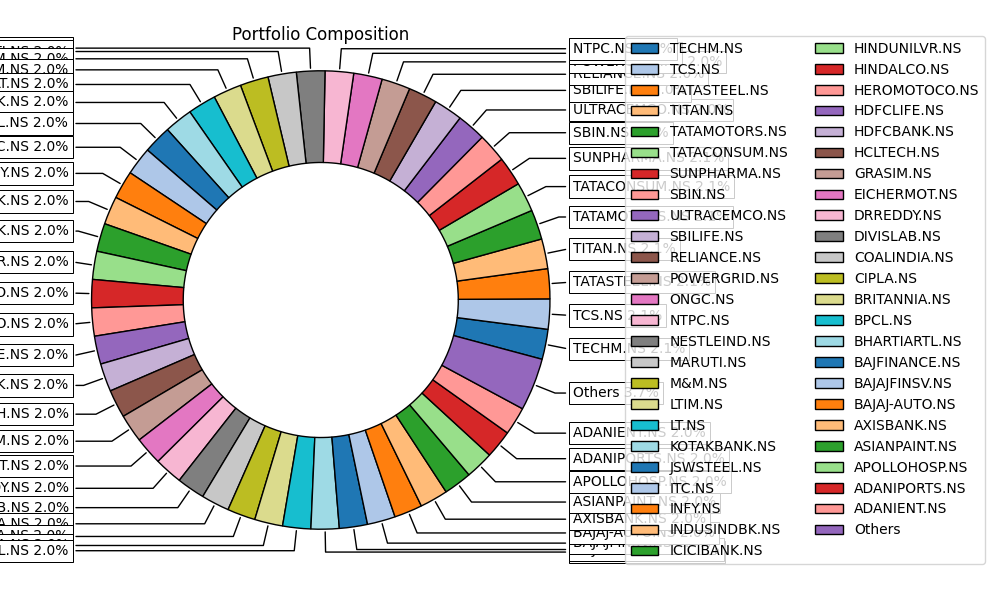
\includegraphics[width=1\linewidth]{images/LSTM/Weights.png}
   \caption{Latest Weights from Optimization}
   \label{fig:network_architecture1}
 \end{figure}

 \begin{figure}[H]
   \centering
   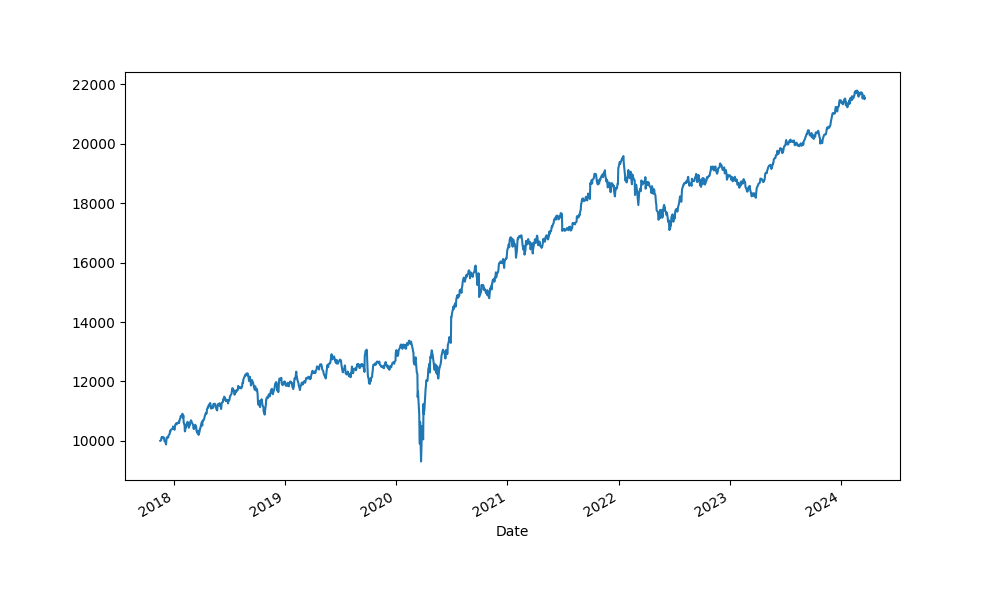
\includegraphics[width=1\linewidth]{images/LSTM/Backtest.png}
   \caption{Backtesting Result}
   \label{fig:network_architecture1}
 \end{figure}

 \begin{table}[H]

    \centering % instead of \begin{center}
    \label{tab:performance_metrics}
    
    \caption{Performace Metrics}
    \vspace{5mm} % Adjust the height of the space between caption and tabular

\begin{tabular}{lr}
\toprule
 & Results \\
\midrule
Expected Return & 18.60\% \\
Volatility & 18.82\% \\
Max Drawdown & -34.89\% \\
Sharpe Ratio & 0.99 \\
Sortino Ratio & 291.92 \\
Omega Ratio & 15.17 \\
CAGR & 18.31\% \\
\bottomrule
\end{tabular}

\end{table}
